\section{Model2DRigid\-Car\-Smooth3Trailers  Class Reference}
\label{class_Model2DRigidCarSmooth3Trailers}\index{Model2DRigidCarSmooth3Trailers@{Model2DRigid\-Car\-Smooth3Trailers}}
A rigid car-like robot with continuous steering angles and three trailers. 


{\tt \#include $<$model2d.h$>$}

Inheritance diagram for Model2DRigid\-Car\-Smooth3Trailers::\begin{figure}[H]
\begin{center}
\leavevmode
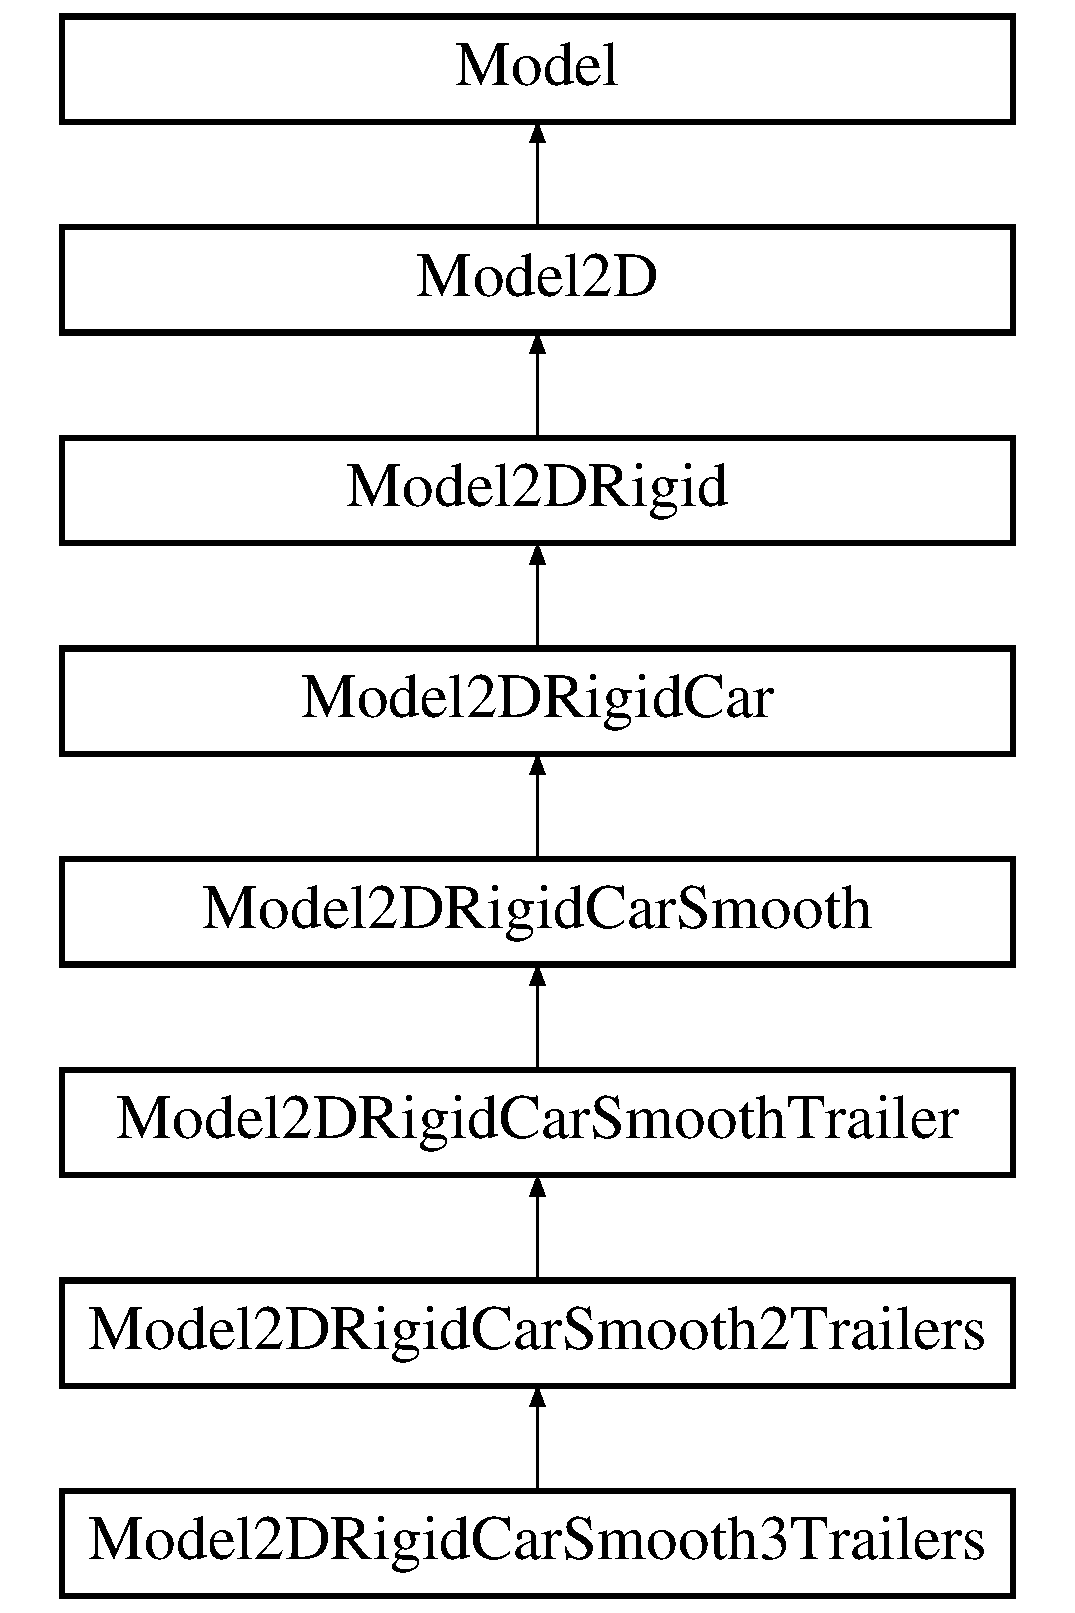
\includegraphics[height=8cm]{class_Model2DRigidCarSmooth3Trailers}
\end{center}
\end{figure}
\subsection*{Public Methods}
\begin{CompactItemize}
\item 
{\bf Model2DRigid\-Car\-Smooth3Trailers} (string path)
\item 
virtual {\bf $\sim$Model2DRigid\-Car\-Smooth3Trailers} ()
\item 
virtual {\bf MSLVector} {\bf State\-Transition\-Equation} (const {\bf MSLVector} \&x, const {\bf MSLVector} \&u)
\begin{CompactList}\small\item\em The state transition equation, or equations of motion, xdot=f(x,u).\item\end{CompactList}\item 
virtual double {\bf Metric} (const {\bf MSLVector} \&x1, const {\bf MSLVector} \&x2)
\begin{CompactList}\small\item\em A distance metric, which is Euclidean in the base class.\item\end{CompactList}\item 
virtual {\bf MSLVector} {\bf State\-To\-Configuration} (const {\bf MSLVector} \&x)
\begin{CompactList}\small\item\em A method that converts a {\bf Model} {\rm (p.\,\pageref{class_Model})} state in to a {\bf Geom} {\rm (p.\,\pageref{class_Geom})} configuration.\item\end{CompactList}\item 
virtual bool {\bf Satisfied} (const {\bf MSLVector} \&x)
\begin{CompactList}\small\item\em Test whether global state-space constraints are satisfied.\item\end{CompactList}\end{CompactItemize}
\subsection*{Public Attributes}
\begin{CompactItemize}
\item 
double {\bf Hitch3Length}
\item 
double {\bf Hitch3Max\-Angle}
\end{CompactItemize}


\subsection{Detailed Description}
A rigid car-like robot with continuous steering angles and three trailers.



\subsection{Constructor \& Destructor Documentation}
\index{Model2DRigidCarSmooth3Trailers@{Model2DRigid\-Car\-Smooth3Trailers}!Model2DRigidCarSmooth3Trailers@{Model2DRigidCarSmooth3Trailers}}
\index{Model2DRigidCarSmooth3Trailers@{Model2DRigidCarSmooth3Trailers}!Model2DRigidCarSmooth3Trailers@{Model2DRigid\-Car\-Smooth3Trailers}}
\subsubsection{\setlength{\rightskip}{0pt plus 5cm}Model2DRigid\-Car\-Smooth3Trailers::Model2DRigid\-Car\-Smooth3Trailers (string {\em path})}\label{class_Model2DRigidCarSmooth3Trailers_a0}


\index{Model2DRigidCarSmooth3Trailers@{Model2DRigid\-Car\-Smooth3Trailers}!~Model2DRigidCarSmooth3Trailers@{$\sim$Model2DRigidCarSmooth3Trailers}}
\index{~Model2DRigidCarSmooth3Trailers@{$\sim$Model2DRigidCarSmooth3Trailers}!Model2DRigidCarSmooth3Trailers@{Model2DRigid\-Car\-Smooth3Trailers}}
\subsubsection{\setlength{\rightskip}{0pt plus 5cm}Model2DRigid\-Car\-Smooth3Trailers::$\sim$Model2DRigid\-Car\-Smooth3Trailers ()\hspace{0.3cm}{\tt  [inline, virtual]}}\label{class_Model2DRigidCarSmooth3Trailers_a1}




\subsection{Member Function Documentation}
\index{Model2DRigidCarSmooth3Trailers@{Model2DRigid\-Car\-Smooth3Trailers}!Metric@{Metric}}
\index{Metric@{Metric}!Model2DRigidCarSmooth3Trailers@{Model2DRigid\-Car\-Smooth3Trailers}}
\subsubsection{\setlength{\rightskip}{0pt plus 5cm}virtual double Model2DRigid\-Car\-Smooth3Trailers::Metric (const {\bf MSLVector} \& {\em x1}, const {\bf MSLVector} \& {\em x2})\hspace{0.3cm}{\tt  [virtual]}}\label{class_Model2DRigidCarSmooth3Trailers_a3}


A distance metric, which is Euclidean in the base class.



Reimplemented from {\bf Model2DRigid\-Car\-Smooth2Trailers} {\rm (p.\,\pageref{class_Model2DRigidCarSmooth2Trailers_a3})}.\index{Model2DRigidCarSmooth3Trailers@{Model2DRigid\-Car\-Smooth3Trailers}!Satisfied@{Satisfied}}
\index{Satisfied@{Satisfied}!Model2DRigidCarSmooth3Trailers@{Model2DRigid\-Car\-Smooth3Trailers}}
\subsubsection{\setlength{\rightskip}{0pt plus 5cm}virtual bool Model2DRigid\-Car\-Smooth3Trailers::Satisfied (const {\bf MSLVector} \& {\em x})\hspace{0.3cm}{\tt  [virtual]}}\label{class_Model2DRigidCarSmooth3Trailers_a5}


Test whether global state-space constraints are satisfied.



Reimplemented from {\bf Model2DRigid\-Car\-Smooth2Trailers} {\rm (p.\,\pageref{class_Model2DRigidCarSmooth2Trailers_a5})}.\index{Model2DRigidCarSmooth3Trailers@{Model2DRigid\-Car\-Smooth3Trailers}!StateToConfiguration@{StateToConfiguration}}
\index{StateToConfiguration@{StateToConfiguration}!Model2DRigidCarSmooth3Trailers@{Model2DRigid\-Car\-Smooth3Trailers}}
\subsubsection{\setlength{\rightskip}{0pt plus 5cm}virtual {\bf MSLVector} Model2DRigid\-Car\-Smooth3Trailers::State\-To\-Configuration (const {\bf MSLVector} \& {\em x})\hspace{0.3cm}{\tt  [virtual]}}\label{class_Model2DRigidCarSmooth3Trailers_a4}


A method that converts a {\bf Model} {\rm (p.\,\pageref{class_Model})} state in to a {\bf Geom} {\rm (p.\,\pageref{class_Geom})} configuration.



Reimplemented from {\bf Model2DRigid\-Car\-Smooth2Trailers} {\rm (p.\,\pageref{class_Model2DRigidCarSmooth2Trailers_a4})}.\index{Model2DRigidCarSmooth3Trailers@{Model2DRigid\-Car\-Smooth3Trailers}!StateTransitionEquation@{StateTransitionEquation}}
\index{StateTransitionEquation@{StateTransitionEquation}!Model2DRigidCarSmooth3Trailers@{Model2DRigid\-Car\-Smooth3Trailers}}
\subsubsection{\setlength{\rightskip}{0pt plus 5cm}virtual {\bf MSLVector} Model2DRigid\-Car\-Smooth3Trailers::State\-Transition\-Equation (const {\bf MSLVector} \& {\em x}, const {\bf MSLVector} \& {\em u})\hspace{0.3cm}{\tt  [virtual]}}\label{class_Model2DRigidCarSmooth3Trailers_a2}


The state transition equation, or equations of motion, xdot=f(x,u).



Reimplemented from {\bf Model2DRigid\-Car\-Smooth2Trailers} {\rm (p.\,\pageref{class_Model2DRigidCarSmooth2Trailers_a2})}.

\subsection{Member Data Documentation}
\index{Model2DRigidCarSmooth3Trailers@{Model2DRigid\-Car\-Smooth3Trailers}!Hitch3Length@{Hitch3Length}}
\index{Hitch3Length@{Hitch3Length}!Model2DRigidCarSmooth3Trailers@{Model2DRigid\-Car\-Smooth3Trailers}}
\subsubsection{\setlength{\rightskip}{0pt plus 5cm}double Model2DRigid\-Car\-Smooth3Trailers::Hitch3Length}\label{class_Model2DRigidCarSmooth3Trailers_m0}


\index{Model2DRigidCarSmooth3Trailers@{Model2DRigid\-Car\-Smooth3Trailers}!Hitch3MaxAngle@{Hitch3MaxAngle}}
\index{Hitch3MaxAngle@{Hitch3MaxAngle}!Model2DRigidCarSmooth3Trailers@{Model2DRigid\-Car\-Smooth3Trailers}}
\subsubsection{\setlength{\rightskip}{0pt plus 5cm}double Model2DRigid\-Car\-Smooth3Trailers::Hitch3Max\-Angle}\label{class_Model2DRigidCarSmooth3Trailers_m1}




The documentation for this class was generated from the following file:\begin{CompactItemize}
\item 
{\bf model2d.h}\end{CompactItemize}
